\chapter{MEASUREMENT OF A MAGIC-ZERO WAVELENGTH}
\label{mzwChapter}

Section \ref{mzwBrief} and Appendix \ref{mzwAppendix} describe our measurement of the first $\lambdaZero$ of potassium, published in \emph{Physical Review Letters} (2012) \cite{Hol12a}. In this chapter I will discuss the relationship between dynamic polarizability, oscillator strengths, and line strengths. I will then discuss our data analysis procedures, derive the fundamental limit to the precision of any $\lambdaZero$ measurement, discuss contrast loss mechanisms, and discuss the effect of an impure optical spectrum on $\lambdaZero$ measurements. Finally, I will discuss several possible new experiments to improve the precision of $\lambdaZero$ measurements. 


\section{Polarizability, oscillator strengths, matrix elements, and all that}
\label{dynPolSec}
The dynamic polarizability $\alpha(\omega)$ can be written most compactly in atomic units as
\begin{eqnarray}
\label{alphaOmegaFeqn}
\alpha(\omega)=\sum_k\frac{f_{k}}{\omega_k^2-\omega^2}
\end{eqnarray}
where $f_k$ is the oscillator strength. Note that the conversion between frequency in atomic and S.I. units is
\begin{eqnarray}
\label{omegaAUSI}
\omega_\textrm{a.u.}&=&\frac{\hbar}{E_h}\omega_\textrm{SI}\nonumber\\
&\approx&\frac{\omega_\textrm{SI}}{4.1341\times10^{16} \textrm{ Hz}} .
\end{eqnarray}
The sum of $f_k$ is approximately equal to the number of valence electrons, i.e.~1 for alkali atoms and 2 for alkaline-earth atoms. $f_k$ is related to the reduced dipole matrix elements through
\begin{eqnarray}
\label{fEqn}
f_k=\frac{2 |\langle \psi || D || \psi_k \rangle|^2 \omega_k}{3(2j+1)}
\end{eqnarray}
where $j$ is the degeneracy of the state of interest, $|\psi\rangle$, and $D$ is the dipole operator. For ground state alkali atoms, $J=1/2$, so $j=2$. We can combine equations \ref{alphaOmegaFeqn} and \ref{fEqn} to write the dynamic polarizability as
\begin{eqnarray}
\label{alphaOmegaMatrixElmEqn}
\alpha(\omega)=\frac{2}{3(2j+1)}\sum_k \frac{|\langle \psi || D || \psi_k \rangle|^2 \omega_k}{\omega_k^2-\omega^2}.
\end{eqnarray}
It is also common to refer to a line strength $S_k = |\langle \psi || D || \psi_k \rangle|^2$. Using this definition, the polarizability becomes
\begin{eqnarray}
\label{alphaOmegaSeqn}
\alpha(\omega)=\frac{2}{3(2j+1)}\sum_k \frac{S_k \omega_k}{\omega_k^2-\omega^2}.
\end{eqnarray}
I have found the conversion of quantities between atomic and S.I. units to be easy to miscalculate and I recommend checking every calculation against a benchmark such as static polarizabilities, transition energies, and literature values of matrix elements. In addition, I recommend keeping a copy of Hilborn's article ``Einstein coefficients, cross sections, f values, dipole moments, and all that" \cite{Hil82} nearby.


So far we have only considered the valence electrons in our polarizability model. Equation \ref{alphaOmegaFeqn} is typically modified to include a core polarizability term, $\alpha_\textrm{core}$, and a valence-core coupling term, $\alpha_\textrm{vc}$:
\begin{eqnarray}
\label{alphaOmegaCore}
\alpha(\omega)=\sum_k\frac{f_{k}}{\omega_k^2-\omega^2} + \alpha_\textrm{core} + \alpha_\textrm{vc}.
\end{eqnarray}
The core and valence-core coupling terms do not have a significant frequency dependence in the optical range. In addition, the valence term is typically broken up into the strongest terms that are explicitly written out with a frequency dependence, plus a ``tail" contribution that is frequency independent and small. When considering the polarizability in the vicinity of the D1 or D2 lines in alkali atoms it is often sufficient to write
\begin{eqnarray}
\label{alphaOmegaTail}
\alpha(\omega)=\frac{f_{D1}}{\omega_{D1}^2-\omega^2} + \frac{f_{D2}}{\omega_{D2}^2-\omega^2} + \alpha_\textrm{tail} + \alpha_\textrm{core} + \alpha_\textrm{vc}.
\end{eqnarray}
The rotating wave approximation, $\omega_{0}^2-\omega^2 \approx 2\omega_0(\omega_0-\omega) = 2\omega_0\Delta$, can also be used to simplify the polarizability near resonance. A factor of $\omega_0$ conveniently cancels in the numerator and the denominator when expressing polarizability near resonance using the line strengths $S_k$:
\begin{eqnarray}
\label{alphaOmegaRWA}
\alpha(\omega)=\frac{2}{3(2j+1)}\sum_k   \frac{S_k}{\Delta_k}.
\end{eqnarray}
Static terms corresponding to tail, core, and valence-core contributions can be added if desired.


Table \ref{kMZWcontTable} summarizes the contributions of each of these parameters near the first magic-zero wavelength of potassium. Uncertainties in the $4s$ to $4p_{1/2}$ (D1) and $4p_{3/2}$ (D2) line strengths dominate the uncertainty of $\lambdaZero$. Our $\lambdaZero$ measurement determines the ratio of these line strengths. Future measurements of additional $\lambdaZero$ in potassium and other atoms will determine different ratios of matrix elements or the core polarizability, depending on the the relative uncertainties of these parameters.



\begin{table}
\caption[Theoretical contributions to the polarizability at the first magic-zero wavelength of potassium.]{\label{kMZWcontTable}Theoretical contributions to the polarizability at $\lambda_\textrm{zero}=769.971$ nm ($\omega_\textrm{zero} = 2\pi\times389.356$ THz), the first magic-zero wavelength of potassium \cite{Saf12per}. Atomic units are used for the matrix elements and the polarizability. The slope of the dynamic polarizability near this $\lambdaZero$ is $\partial \alpha / \partial \lambda = -42500$ $a_0^3$/nm and the uncertainty in the polarizability near this $\lambdaZero$ is 100 $a_0^3$. This results in a theoretical uncertainty in $\lambdaZero$ of $\delta\lambdaZero = (\partial \alpha/ \partial \lambda)|^{-1}_{\lambda\textrm{zero}} \delta\alpha(\lambdaZero)= 2.5$ pm.}
\begin{center}
\begin{tabular}{l c r}
\hline\hline
Contribution & $|\langle 4s_{1/2} || D || np_{1/2} \rangle|$ & $\alpha(\omega_\textrm{zero})$ \\
\hline
$4p_{1/2}$ & 4.106(6) & -32085(62) \\
$4p_{3/2}$ & 5.807(7) & 32079(77) \\
$5p_{1/2}$ & 0.271(5) & 0.30(1) \\
$5p_{3/2}$ & 0.398(8) & 0.65(2) \\
$\alpha_\textrm{tail}$ & & 0.16(12) \\
$\alpha_\textrm{core}$ & & 5.46(27)\\
$\alpha_\textrm{vc}$ & & -0.18(1) \\
\hline
$\alpha_\textrm{total}$ & & 0(100)\\
\end{tabular}
\end{center}
\end{table}



As stated previously, the energy shift of a polarizable atom is given by 
\begin{eqnarray}
U(\omega) = -\frac{1}{2} \alpha(\omega) \vec{E}^2(\omega,z,t)
\end{eqnarray}
where we now allow for a frequency dependence for the polarizability and the electric field. For optical frequencies, we can only measure the energy shift due to the time average of the electric field, i.e.~the intensity. The intensity is related to the electric field amplitude by $I=c\epsilon_0 |E|^2/2$. From this, we can find that the phase acquired along one interferometer path is given by $\alpha(\omega)$ and the intensity of the light $I(x,z)$ at that location:
\begin{eqnarray}
\label{mzwIntEqn}
\phi_0(\omega) = \frac{\alpha(\omega)}{2\epsilon_0 c \hbar v}\int_{-\infty}^{\infty}I(x,z) dz.
\end{eqnarray}
Similar to the static polarizability experiment, where we used a static electric field gradient, here, we use an intensity gradient to apply different phase shifts to each interferometer path. We measure the differential phase shift of the two interferometer paths. Measurements of these differential phase shifts as a function of optical frequency, or wavelength, let us determine $\lambdaZero$.





\section{Data analysis procedures}
\label{mzwDataAnalysis}
In this section we will describe in detail how we processed approximately 12,000 atom interferometer fringes (the result of about 6 billion atoms) to ultimately report our precision measurement of $\lambda_\textrm{zero}$. 


We measured atom interferometer fringes in 5 s chunks of data and fit these fringes to determine the interferometer phase and contrast \cite{Ber97,Cro09}. During each 5 s of data, the measured atom beam flux was typically $10^5$ counts/s and the measured fringe contrast was typically 25\%. We used a mechanical shutter to alternately measure the interferometer fringes with and without laser light. The interferometer phase drifted at a rate of about 5 rad/hr, due primarily to thermal fluctuations of the apparatus. We fit the light-off reference phase to a smoothing spline and then subtracted the spline from the light-on phase to determine the interferometer phase shift. Figure \ref{MZWRefOnPhase} shows the measured laser power, laser wavelength, phase shift, reference phase residuals, and contrast for each 5 s data file during a 30 min measurement of $\lambda_\textrm{zero}$. The statistical uncertainties of the contrast and phase were determined by the $\chi^2$ minimization algorithm (reduced $\chi^2$ values were typically 1.2-1.4). Unfortunately, the interferometer phase was less stable than the precision that each data file suggested that it should be, and this is ultimately the dominate source of statistical uncertainty in our experiment. Improving the interferometer stability is a long-standing goal of our lab. Changing the parameters of the smoothing spline can result in a random change of up to several picometers to the best-fit $\lambda_\textrm{zero}$ of most of the individual data series but does not significantly alter the overall average $\lambda_\textrm{zero}$.


\begin{figure}
\centerline{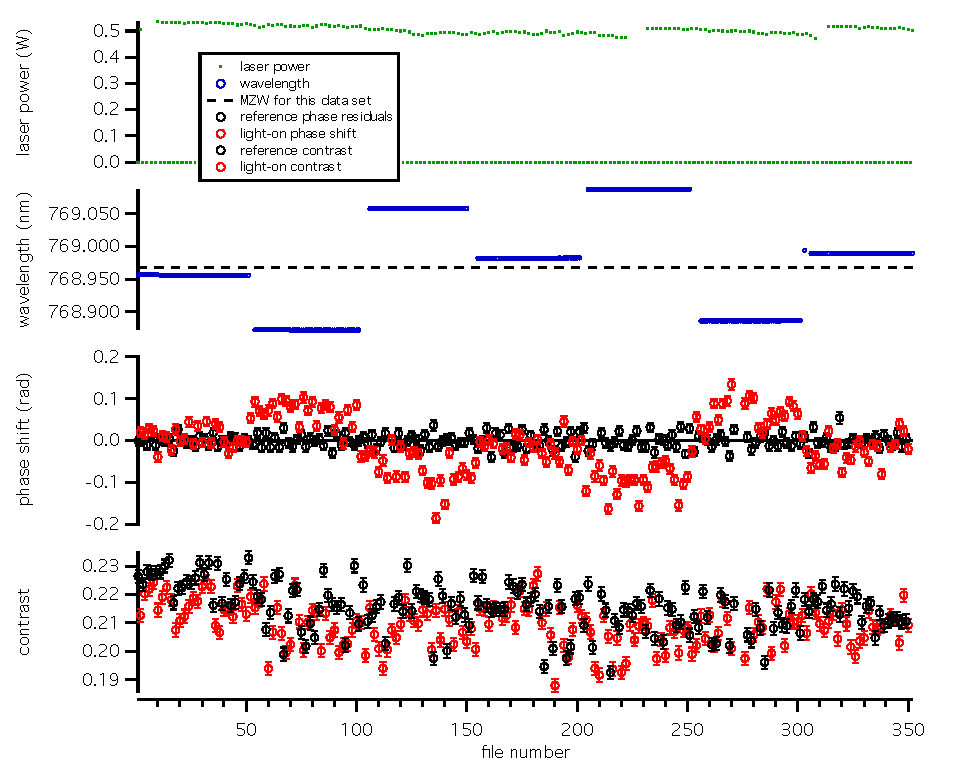
\includegraphics[width=.90\textwidth]{Figures/120509eRefOnPhaseWavePowerCon.pdf}}
\caption[Light-induced phase shift and contrast, and laser power and wavelength vs.~data file number]{\label{MZWRefOnPhase}Laser power, laser wavelength, reference atom interferometer phase residuals and contrast, and light-induced atom interferometer phase shift and contrast vs.~data file number. Each data point corresponds to 5 s of integration time. 29 out of 350 data points were deleted in this data set due to instabilities in either the laser power or wavelength during the 5 s integration time, and the phase shift data is ignored for these files. These deletions are accomplished using an unbiased and automated filter algorithm. These data are then further analyzed by normalizing the phase shift data by the laser power, and then binning and averaging the normalized phase shift data by wavelength, as shown in Figure \ref{MZWphaseVsWave}. The particular data shown here is data set 120509e.}
\end{figure}


After the initial data processing, we normalized the phase shift data by laser power to control for drifts of the tapered amplifier power and fiber coupling efficiency. In addition, polarization changes due to propagation through the fiber were converted to power instability by a polarizing beam splitter. The power-normalized phase shift data were then binned by wavelength, and the average, standard deviation, and standard error of the mean of the central 80\% of each bin was calculated. Figure \ref{MZWphaseVsWave} shows the resulting average power-normalized phase shift data vs.~wavelength. We performed a non-linear least-squares fit of this data to equation 4 from Appendix \ref{mzwAppendix} to determine the $\lambda_\textrm{zero}$ for each data series. For this fit, we weighted the normalized phase shift data by the standard error of the mean for each wavelength bin. The statistical error of each $\lambda_\textrm{zero}$ measurement was determined by the fit routine. The standard deviation is only shown for reference. The quality of fit shown in Figure \ref{MZWphaseVsWave} is typical of the entire data set. 


\begin{figure}
\centerline{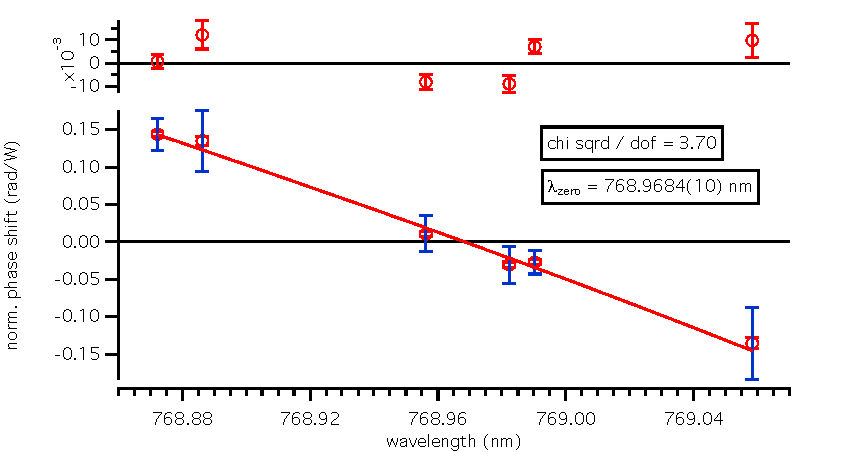
\includegraphics[width=.90\textwidth]{Figures/120509eMZWmeas.pdf}}
\caption[Power-normalized average phase shift vs.~wavelength for data series 120509e.]{\label{MZWphaseVsWave}Power-normalized average phase shift vs.~wavelength for data series 120509e. The red error bars are the standard error of the mean and the blue error bars are the standard deviation of the phase shifts measured at each wavelength. The 1.0 pm best-fit uncertainty of $\lambda_\textrm{zero}$ in this data series comes from $\chi^2$ minimization using input uncertainties of the standard error of the mean of the averaged phase shifts at each wavelength. The $\lambda_\textrm{zero}$ reported from this data series is compared to 34 other measurements each made in a similar way in Figure \ref{MZWmeasFig}.}
\end{figure}


Our reported $\lambda_\textrm{zero}$ measurement is the result of 35 individual measurements of $\lambda_\textrm{zero}$, such as the one shown in Figure \ref{MZWphaseVsWave}. Each $\lambda_\textrm{zero}$ measurement and an estimate of its statistical uncertainty is shown in Figure \ref{MZWmeasFig}. A histogram of the 35 measurements is shown in Figure \ref{MZWhistFig}. Note that these measurements have not been corrected for a constant Doppler shift of 0.56(5) pm. 


The reproducibility of the 35 $\lambda_\textrm{zero}$ measurements shown in Figure \ref{MZWmeasFig} is clearly much worse than the individual statistical errors. Furthermore, even the relative sizes of the individual statistical errors appear highly suspect since the reproducibility of the measurements i.e. the deviation from the mean, is uncorrelated with the size of the statistical errors. We therefore chose to assume that the statistical error of each data set was the same. We do not feel justified taking the weighted mean of these measurements because we do not believe the statistical errors associated with the each of the 35 individual measurements are accurate.


\begin{figure}
\centerline{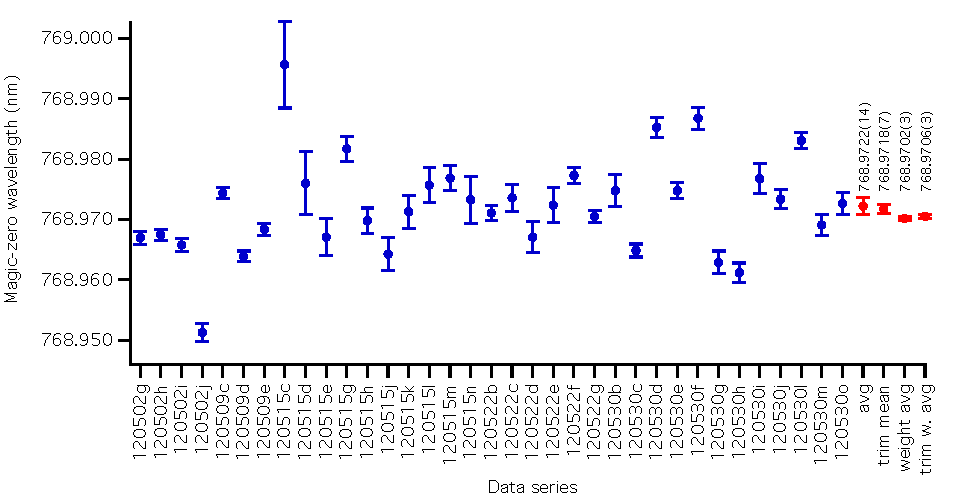
\includegraphics[width=.90\textwidth]{Figures/MZWmeasurements2.pdf}}
\caption[35 separate $\lambda_\textrm{zero}$ measurements and the average calculated in 4 different ways.]{\label{MZWmeasFig}35 separate $\lambda_\textrm{zero}$ measurements (blue) and the average calculated in 4 different ways (red). The overall average is $\lambda_\textrm{zero}=768.9722(14)$, the average of the central 80\% of the data is $\lambda_\textrm{zero}=768.9718(7)$ nm, the weighted overall average is $\lambda_\textrm{zero}=768.9702(3)$ nm, and the weighted average of the central 80\% of the data is $\lambda_\textrm{zero}=768.9706(3)$ nm. The error bars for each individual measurement show the uncertainty that was determined by $\chi^2$ minimization. However, as shown here, we found the experiment was not as reproducible as the reported individual measurement errors would suggest. Furthermore, the deviation from the mean was also uncorrelated with the size of the statistical error. Therefore, we assumed the statistical errors of all measurements were the same, and we report the standard error of the trimmed mean as the final statistical uncertainty. This data has not been corrected for a 0.56(5) pm Doppler shift. Figure \ref{MZWhistFig} shows a histogram of these data.}
\end{figure}


If we take the average of all 35 measurements and calculate the standard error of the mean, we find $\lambda_\textrm{zero}=768.9722(14)$ nm. Eliminating the highest and lowest 10\% of the data yields the reported measurement of $\lambda_\textrm{zero}=768.9718(7)$ nm (again, without the Doppler shift correction). The weighted average of all 35 points is $\lambda_\textrm{zero}=768.9702(3)$ nm, and the weighted average of the central 80\% of the data is $\lambda_\textrm{zero}=768.9706(3)$ nm. The statistical errors associated with the weighted averages are unrealistically small, yet, the central values are within 1.2 pm (2$\sigma$) of unweighted averages. 

\begin{figure}
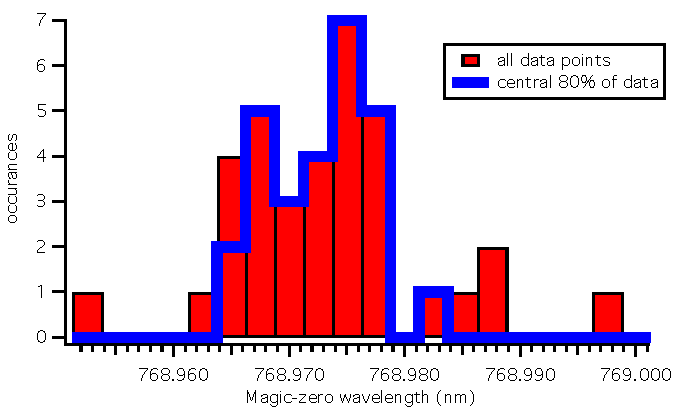
\includegraphics[width=.90\textwidth]{Figures/MZWhistogram.pdf}
\caption[Histogram of $\lambda_\textrm{zero}$ measurements.]{\label{MZWhistFig}Histogram of $\lambda_\textrm{zero}$ measurements. The central 80\%, used for the calculation of the trimmed mean, is highlighted in blue.}
\end{figure}





\section{Derivation of a fundamental limit for the sensitivity of a $\lambdaZero$ measurement}
\label{mzwLimitSection}
Decoherence due to spontaneous emission \cite{Cha95, Kok01a} limits the precision with which $\lambda_\textrm{zero}$ can be measured. The probability of an atom scattering zero photons, $P(0)$, affects the interferometer contrast through $C=C_0P(0)$, where $C_0$ is the reference contrast. Given a Poisson distribution for $P(0)$,
\begin{eqnarray}
\label{ceqn}
C = C_0 e^{-N(\omega)}
\end{eqnarray}
where $N(\omega)$ is the average number of photons an atom scatters while exposed to the laser beam with frequency $\omega$ for a time $T$. $N(\omega)$ is proportional to the time-averaged probability for atoms to be in an excited state, $P_{ex}$, and the decay rate $\Gamma$: 
\begin{eqnarray}
&N(\omega)=&P_{ex} T \Gamma.
\end{eqnarray}
When the excitation probability is much less than 1, and using the rotating wave approximation, we can write $P_{ex}$ in terms of the Rabi frequencies $\Omega_e=|\langle e | \bm{d} . \bm{\hat{\epsilon}} | g \rangle |E_0/\hbar$ and the detunings $\Delta_e$ from each resonance:
\begin{eqnarray}
\label{PexEqn}
P_{ex}=\frac{1}{2} \sum_e \frac{\Omega_e^2}{\Delta_e^2+\Omega_e^2}
\end{eqnarray}

The probability of an atom scattering 1 or more photons is $P_s=1-P(0)$. To obtain a simple expression for $P_s$ we make the approximation
\begin{eqnarray}
\label{P0eqnApprox}
P(0) \approx 1-N(\omega)
\end{eqnarray}
Using this approximation, we can write
\begin{eqnarray}
\label{psEqn}
P_s = N(\omega) = P_{ex}T\Gamma = T\Gamma \frac{1}{2} \sum_e \frac{\Omega_e^2}{\Delta_e^2+\Omega_e^2}.
\end{eqnarray}
To compare $P_s$ to the phase shift, we further assume $\Delta_e^2 \gg \Omega_e^2$ and rewrite $P_s$ as
\begin{eqnarray}
\label{psMatrixElEqn}
P_s = P_{ex}T\Gamma = \frac{I T\Gamma}{\epsilon_0 c \hbar^2} \sum_e \frac{|\langle e | \bm{d} . \bm{\hat{\epsilon}} | g \rangle |^2}{\Delta_e^2}.
\end{eqnarray}
In the rotating-wave approximation, the slope of the phase shift is
\begin{eqnarray}
\label{rwaPhaseDer}
\frac{d\phi}{d\omega}=\frac{IT}{2\epsilon_0c\hbar^2} \sum_e \frac{|\langle e | \bm{d} . \bm{\hat{\epsilon}} | g \rangle | ^2}{\Delta_e^2}.
\end{eqnarray}

Comparison of Eqs.~(\ref{rwaPhaseDer}) and (\ref{psMatrixElEqn}) yields a maximum achievable slope of
\begin{eqnarray}
\label{OmegaLimit}
\frac{d\phi}{d\omega}\approx\frac{1}{2\Gamma}P_s.
\end{eqnarray}
In terms of the wavelength, the slope is
\begin{eqnarray}
\label{LambdaLimit}
\frac{d\phi}{d\lambda}=\frac{d\phi}{d\omega}\frac{d\omega}{d\lambda}\approx\frac{\pi c P_s}{\lambda^2\Gamma}.
\end{eqnarray}

As discussed in Appendix \ref{mzwAppendix}, the highest sensitivity could be achieved if $P_0=e^{-1}$, implying an optimum $P_s=1-e^{-1}$. Given this requirement, we determine that the error made by the approximation in Eq.~(\ref{P0eqnApprox}) is $\approx30\%$. Still, the simple formulation of the maximum achievable slope presented in Eq.~(\ref{OmegaLimit}) remains a useful guide to possibility of large improvements in the precision of $\lambda_\textrm{zero}$ measurements. 




\section{Contrast loss due to inhomogeneous mechanisms}
\label{mzwContrast}

Although the phase shift is the primary signal in our measurement of $\lambda_\textrm{zero}$, it is still important to have a full understanding of the interferometer contrast loss. This provides a valuable check on our understanding of the potential errors associated with the measurement. Here we will examine three mechanisms of contrast loss, all analogous to inhomogenous broadening.

As stated in equation \ref{mzwIntEqn}, the phase acquired along one path in the atom interferometer is
\begin{eqnarray}
\label{inteqnEPAPS}
\phi_{0,q,|Fm_F\rangle}(\omega,x,v) = \frac{\alpha_{q,|Fm_F\rangle}(\omega)}{2\epsilon_0 c \hbar v}\int_{-\infty}^{\infty}I(x,z) dz.
\end{eqnarray}
Here we have written the phase as an explicit function of the atom wave position $x$, velocity $v$, light polarization $q$, and state $|Fm_F\rangle$ to more easily explain the contrast loss mechanisms. Next, we assume that the focused laser beam intensity distribution in the plane of the interferometer is represented by a Gaussian function
\begin{eqnarray}
\label{intensityEqnEPAPS}
I(x_l,z_l) = I_{0}e^{-2(x_l^2+z_l^2)/w_0^2}
\end{eqnarray}
where $w_0$ is the beam waist, $I_{0}=2P_L/(\pi w_0^2)$ and $P_L$ is the laser power. Integrating the acquired phase (Eq.~(\ref{inteqnEPAPS})) along the beam path ($z$) gives
\begin{eqnarray}
\label{nointeqniEPAPS}
\phi_{0,q,|Fm_F\rangle}(\omega,x,v) = \frac{\alpha_{q,|Fm_F\rangle}(\omega)\sqrt{\pi/2}w_0I_{0}}{2\epsilon_0 c \hbar v}e^{-2(x-x_l)^2/w_0^2},
\end{eqnarray}
or in terms of the laser power and beam waist
\begin{eqnarray}
\label{nointeqnpEPAPS}
\phi_{0,q,|Fm_F\rangle}(\omega,x,v)=\frac{\alpha_{q,|Fm_F\rangle}(\omega)P_L}{\sqrt{2\pi}\epsilon_0 c \hbar v w_0}e^{-2(x-x_l)^2/w_0^2}.
\end{eqnarray}


The differential phase shift between the two paths of the two interferometers formed by the +1 and 0, and the 0 and -1 diffraction orders is
\begin{subequations}
\label{diffPhaseEPAPS}
\begin{eqnarray}
\phi_{1,q,|Fm_F\rangle}(\omega,x,v) = \phi_{0,q,|Fm_F\rangle}(\omega,x+s(v),v)-\phi_{0,q,|Fm_F\rangle}(\omega,x,v)\\
\phi_{-1,q,|Fm_F\rangle}(\omega,x,v) = \phi_{0,q,|Fm_F\rangle}(\omega,x,v)-\phi_{0,q,|Fm_F\rangle}(\omega,x-s(v),v)
\end{eqnarray}
\end{subequations}
where $s(v)$ is the velocity-dependent path separation \cite{Hol10}. 


The velocity distribution in our supersonic atom beam is well-described by a Gaussian distribution
\begin{eqnarray}
\label{PveqnEPAPS}
P(v)=\frac{1}{\sqrt{2\pi\sigma_v^2}}\exp\left(-\frac{(v-v_0)^2}{2\sigma_v^2}\right)
\end{eqnarray}
where $v_0$ is the mean velocity and $\sigma_v$ is the velocity distribution width. In our experiment $v_0\approx1600$ m/s and $v_0/\sigma_v\approx15$.


Finally, we can predict the measured interferometer phase $\phi(\omega)$ and contrast $C(\omega)$ from the expression
\begin{eqnarray}
\label{cphiEPAPS}
C(\omega)e^{i\phi(\omega)}=C_0e^{i\phi_0}\sum_{q=-1,0,1}f_q\sum_{k=-1,1}\frac{1}{2}\sum_{|Fm_F\rangle}\frac{1}{8}\int_{v=0}^\infty P(v)\int_{x=-d/2}^{d/2}\nonumber\\
P(x)\exp(i\phi_{k,q,|Fm_F\rangle}(\omega,x,v)) dv dx.
\end{eqnarray}
Here, $f_q$ is the fraction of the power with $q$ polarization, typically $f_{0}=80\%$ and $f_{1}=20\%$. The factor of 1/2 accounts for equal detected intensity from the +1 and -1 interferometers. The factor of 1/8 accounts for the fact that all 8 $|Fm_F\rangle$ states are equally likely in our thermal atom beam. We also assume that the atom beam intensity $P(x)=1/d$ is uniform over the width $d$ of the detected fringes. Figure \ref{MZWcLossFig} shows contrast loss spectra based on Eq.~\ref{cphiEPAPS} with several conditions (e.g. zero beam width). Figure 1b in Appendix \ref{mzwAppendix} shows the same data and the calculated contrast loss spectra for the conditions $d=100$ $\mu$m, $\sigma_v=110$ m/s, $w_0=110$ $\mu$m. 


\begin{figure}
\centerline{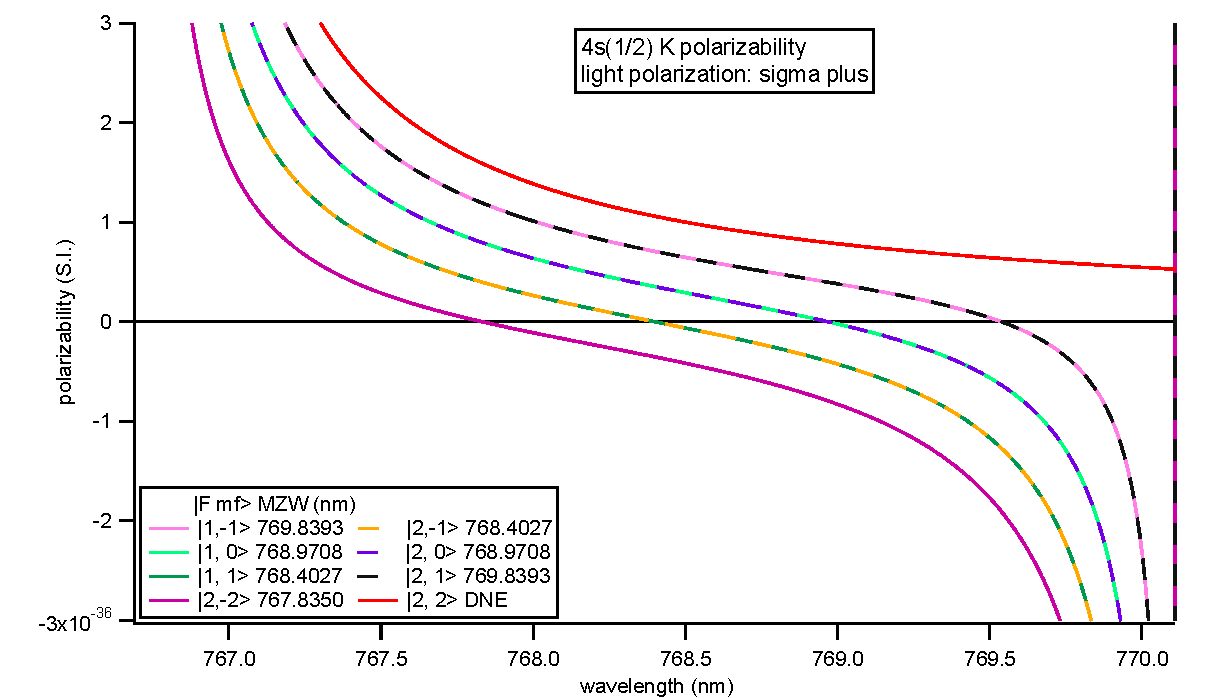
\includegraphics[width=.90\textwidth]{Figures/sigmaPlusMZW.pdf}}
\caption{\label{sigmaPlusMZW}Polarizabilities and magic-zero wavelengths for different $|Fm_F\rangle$ ground states of potassium for $\sigma^+$ light.}
\end{figure}


\begin{figure}
\centerline{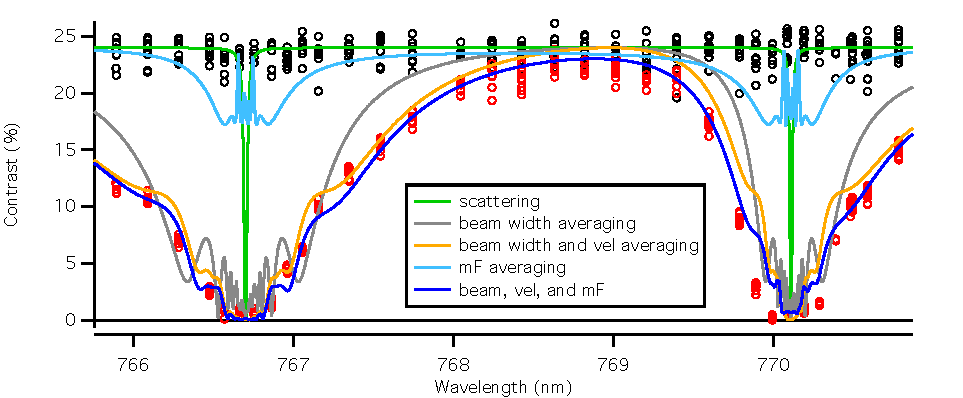
\includegraphics[width=1\textwidth]{Figures/cLossMechanisms.pdf}}
\caption[Interferometer contrast loss due to light between the potassium D1 and D2 lines.]{\label{MZWcLossFig}Measured interferometer reference contrast $C_0$ (black circles) and contrast $C$ when exposed to light (red circles). Also shown is predicted interferometer contrast loss due to averaging over the beam width only (grey line), the beam width and the velocity distribution (orange line), multiple $|Fm_F\rangle$ states only (light blue line), and all three of the above mechanisms (dark blue line). Contrast loss from photon scattering only is also shown (green line).}
\end{figure}



\section{The effect of broadband light on $\lambdaZero$ measurements}

We have assumed, until now, that the optical spectrum contains only one frequency of significance. Unfortunately, due to the nature of our laser system, this assumption is not valid. Our laser system consists of tunable a 50 mW external cavity diode laser seeding a 2 W tapered amplifier \cite{Haw01, Bol10, Nym06}. Tapered amplifiers are notorious for producing a significant amount of broadband spontaneous emission ($\sim10\%$ of the total power output) in addition to the amplified stimulated emission. Figure \ref{ASEgratingPic} shows a picture of the spectrum of the tapered amplifier power output after diffraction from a grating. Figure \ref{mzwSponData} shows data acquired with a grating spectrometer under different TPA conditions. Under normal operating conditions (40 mW of seed light and a TPA current of 2.6 A) the broadband light spectrum is consistent with a gaussian with a center wavelength of $\lambda_\textrm{spon}=763$ nm and a width of $\sigma_\textrm{spon}=3$ nm. Spontaneous emission from the tapered amplifier diverges at a different rate than the stimulated emission. We use this fact to reduce the fraction of spontaneous emission by an order of magnitude by spatially filtering the tapered amplifier output with a single mode fiber \cite{Voi01}. 


To account for the broadband light, the phase shift (equation \ref{mzwIntEqn}) becomes
\begin{eqnarray}
\label{mzwIntEqnASE}
\phi(\omega) = \frac{1}{\epsilon_0 c \hbar v} \int_{z=-\infty}^{\infty} \int_{\omega=0}^{\infty} \alpha(\omega)  I(\omega;x,z) dz d\omega.
\end{eqnarray}
Figure \ref{mzwSponSpectrum} shows a model of the broadband light spectrum with the dynamic polarizability near the potassium D1 and D2 lines.


\begin{figure}
\centerline{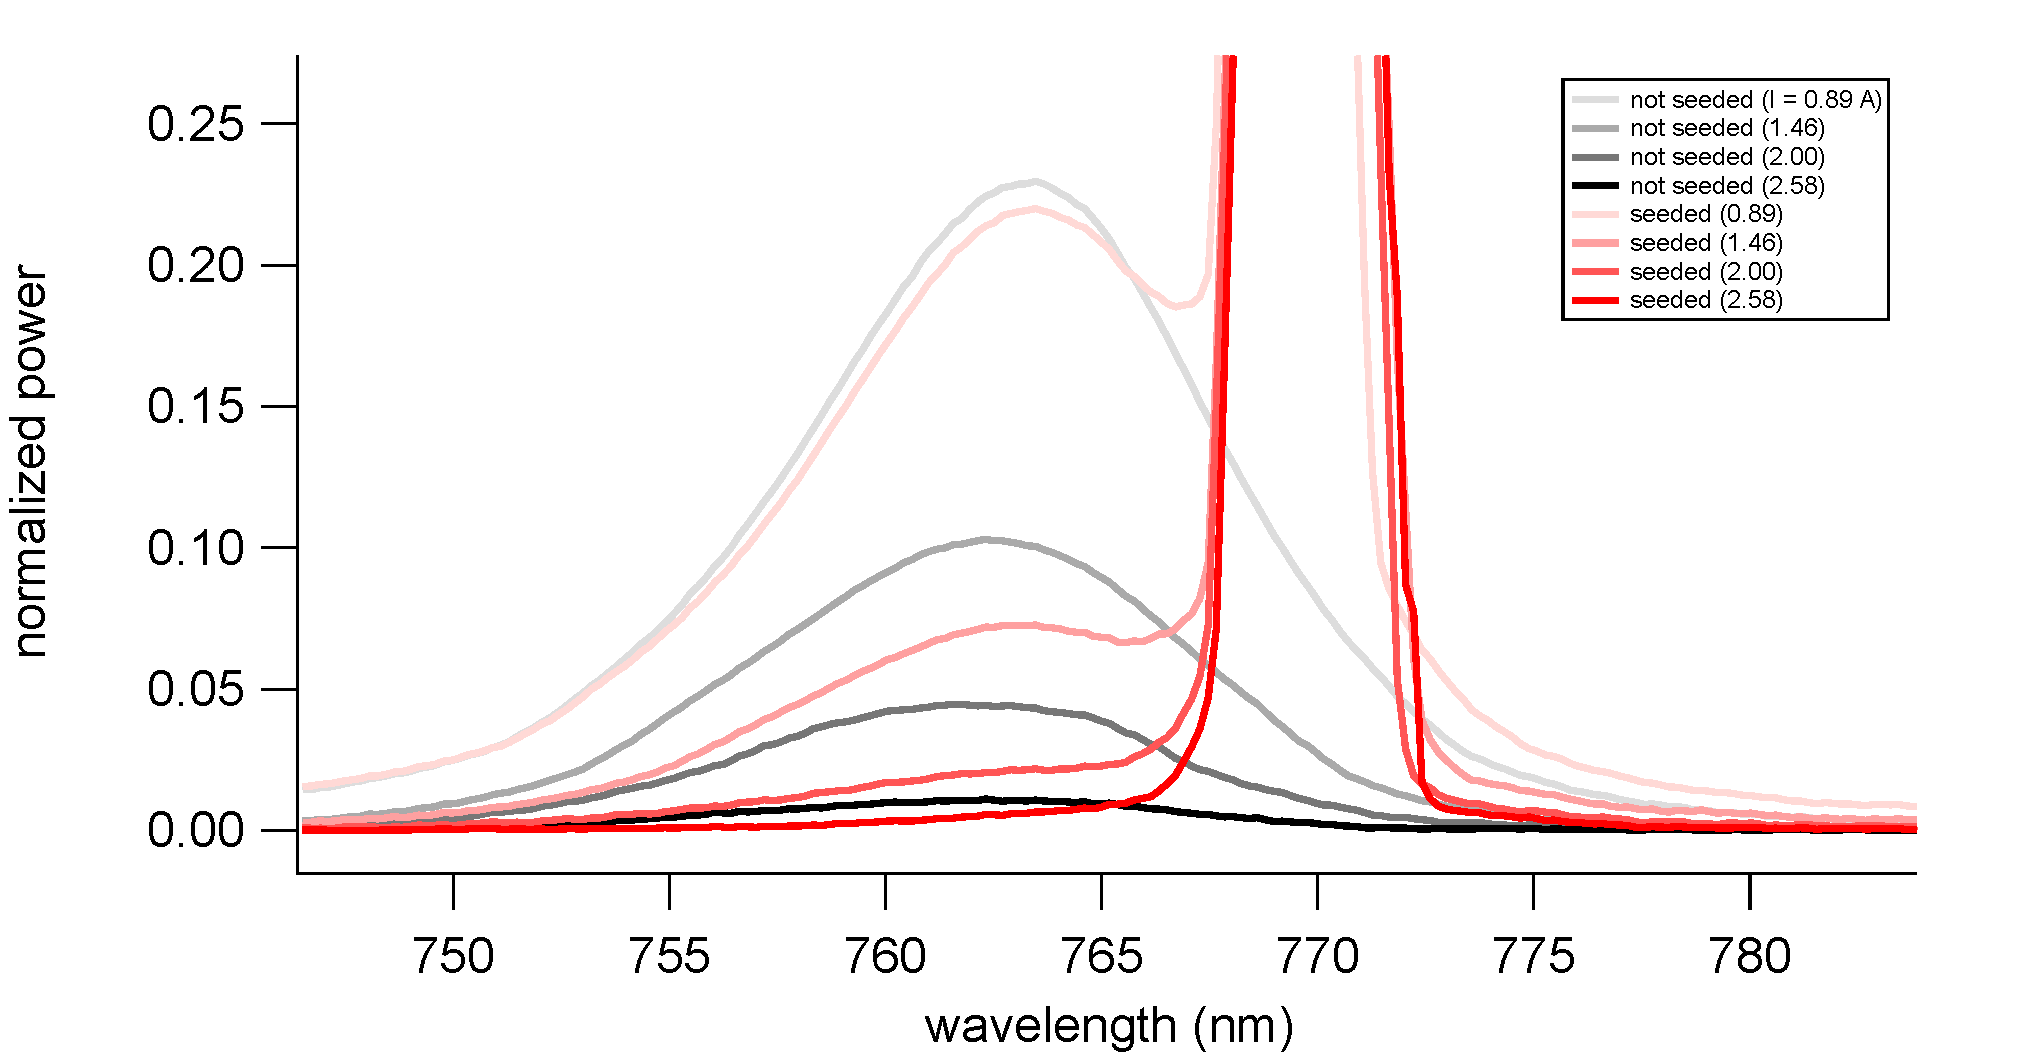
\includegraphics[width=.9\textwidth]{Figures/ASEdata.pdf}}
\caption[Laser spectrum measured with a grating spectrometer.]{\label{mzwSponData}Laser system spectrum before filtering by a single mode fiber for 4 different tapered amplifier injection currents: 0.89 A, 1.46 A, 2.00 A, and 2.58 A. Black curves are the unseeded tapered amplifier spectrum (spontaneous emission only). Red curves are the spectrum when the tapered amplifier is seeded. The darkness gradient corresponds to low (faint) to high (dark) currents. For each of the 4 currents, both the unseeded and seeded spectrum is normalized so that the maximum observed power is equal to 1. Thus it is evident that as the tapered amplifier injection current increases, the broadband light component decreases. The grating spectrometer resolution is approximately 0.3 nm, and this causes a blurring of the high power stimulated emission peak.}
\end{figure}


\begin{figure}
\centerline{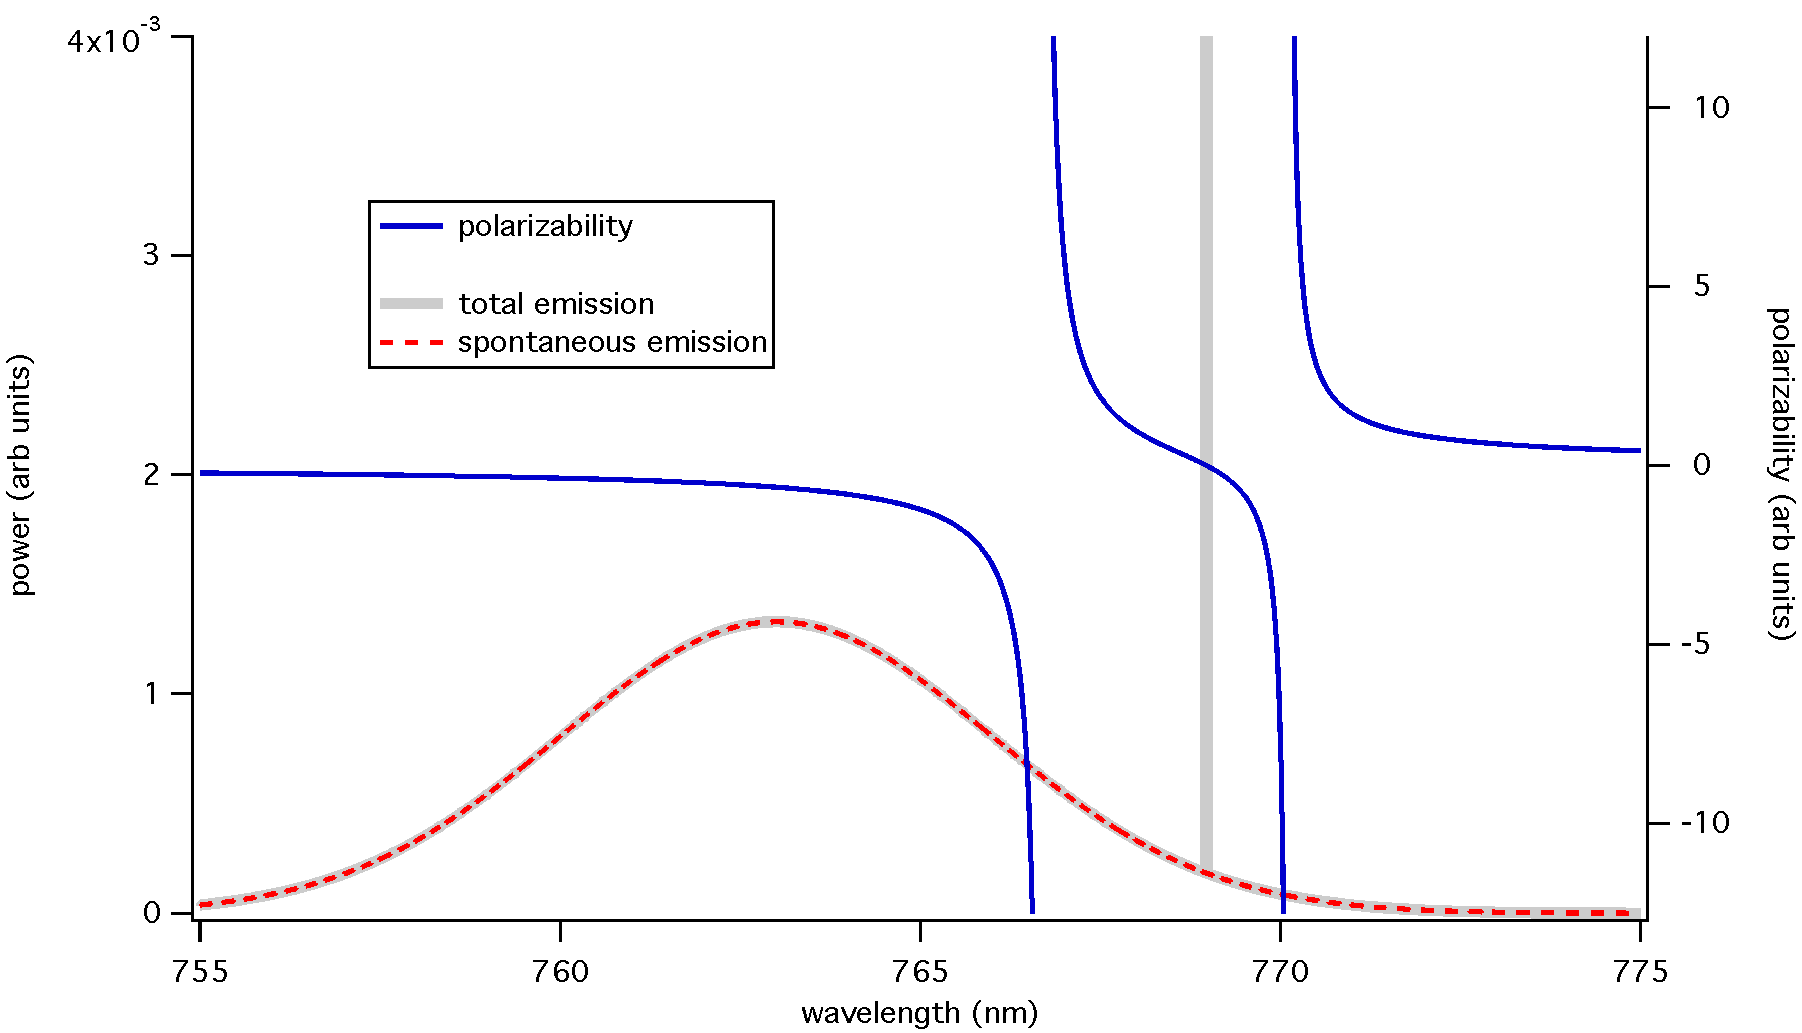
\includegraphics[width=.9\textwidth]{Figures/ASEmodelSpectrum2.pdf}}
\caption[Plot of the laser spectrum and the dynamic polarizability of potassium.]{\label{mzwSponSpectrum}Model of the laser system spectrum and the dynamic polarizability of K. The  broadband light component is set to be 1\% of the total laser power. The majority of the broadband light is blue-detuned of the D2 line, and thus there is a net phase shift due to the integrated spectral density of the broadband light.}
\end{figure}




%%%%%%%%%%%%%%%%%%%%%%%%%%%%%%%
\section{Next-generation $\lambdaZero$ measurements}
\label{mzwNextGenSec}
The existence of a $\lambdaZero$ near 770 nm in potassium was fortunate for our lab. We chose to study this particular $\lambdaZero$ for several reasons. First, potassium is cheap and easy to handle, and it is easy to generate and detect beams of potassium atoms in our lab. Second, the primary transitions are strong and the fine structure splitting of the $4p$ levels in potassium is only 3 nm, and this leads to a larger slope and thus easier to determine $\lambdaZero$. Third, inexpensive and easy-to-operate diode lasers and amplifiers are available near 770 nm.

Future measurements of magic-zero wavelengths in our lab will not have all of these advantages. Therefore, we are exploring ways to increase the light-induced phase shift in our atom interferometer and improve the reproducibility of the measurements. Three ideas to improve the signal size are a ``hall of mirrors" (Figure \ref{mzwHOM}), a power build-up cavity (Figure \ref{mzwCavityFig}), and a coaxial atom-light interaction region (Figure \ref{mzwHoleyMirror}). All of these ideas would rely on light delivered into the vacuum chamber by a single-mode optical fiber, and all optics would be rigidly attached to improve the stability and reproducibility of the experiment. 

We have already built a hall of mirrors and used it to measure the same $\lambdaZero$. The slope $d\phi/d\lambda$ is as much as 10 times larger as in our published experiment. Furthermore, the reproducibility during a single day is also improved and now consistent with the statistical error of a single $\lambdaZero$ measurement. We attribute this improvement in reproducibility to the increased mechanical robustness of the hall of mirrors system.

\begin{figure}
\centerline{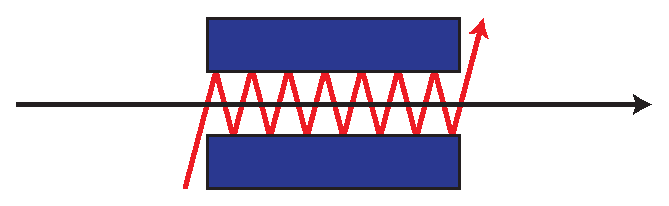
\includegraphics[width=.90\textwidth]{Figures/HOM.eps}}
\caption[A hall-of-mirrors for improved measurements of $\lambdaZero$.]{\label{mzwHOM}A ``hall-of-mirrors" for improved measurements of $\lambdaZero$. A hall-of-mirrors allows the laser beam to intersect the atom beam multiple times to create a larger phase shift. Nearly parallel mirrors and an appropriate choice of the focusing power of the lens may result in 30-50 times larger phase shifts.}
\end{figure}

\begin{figure}
\centerline{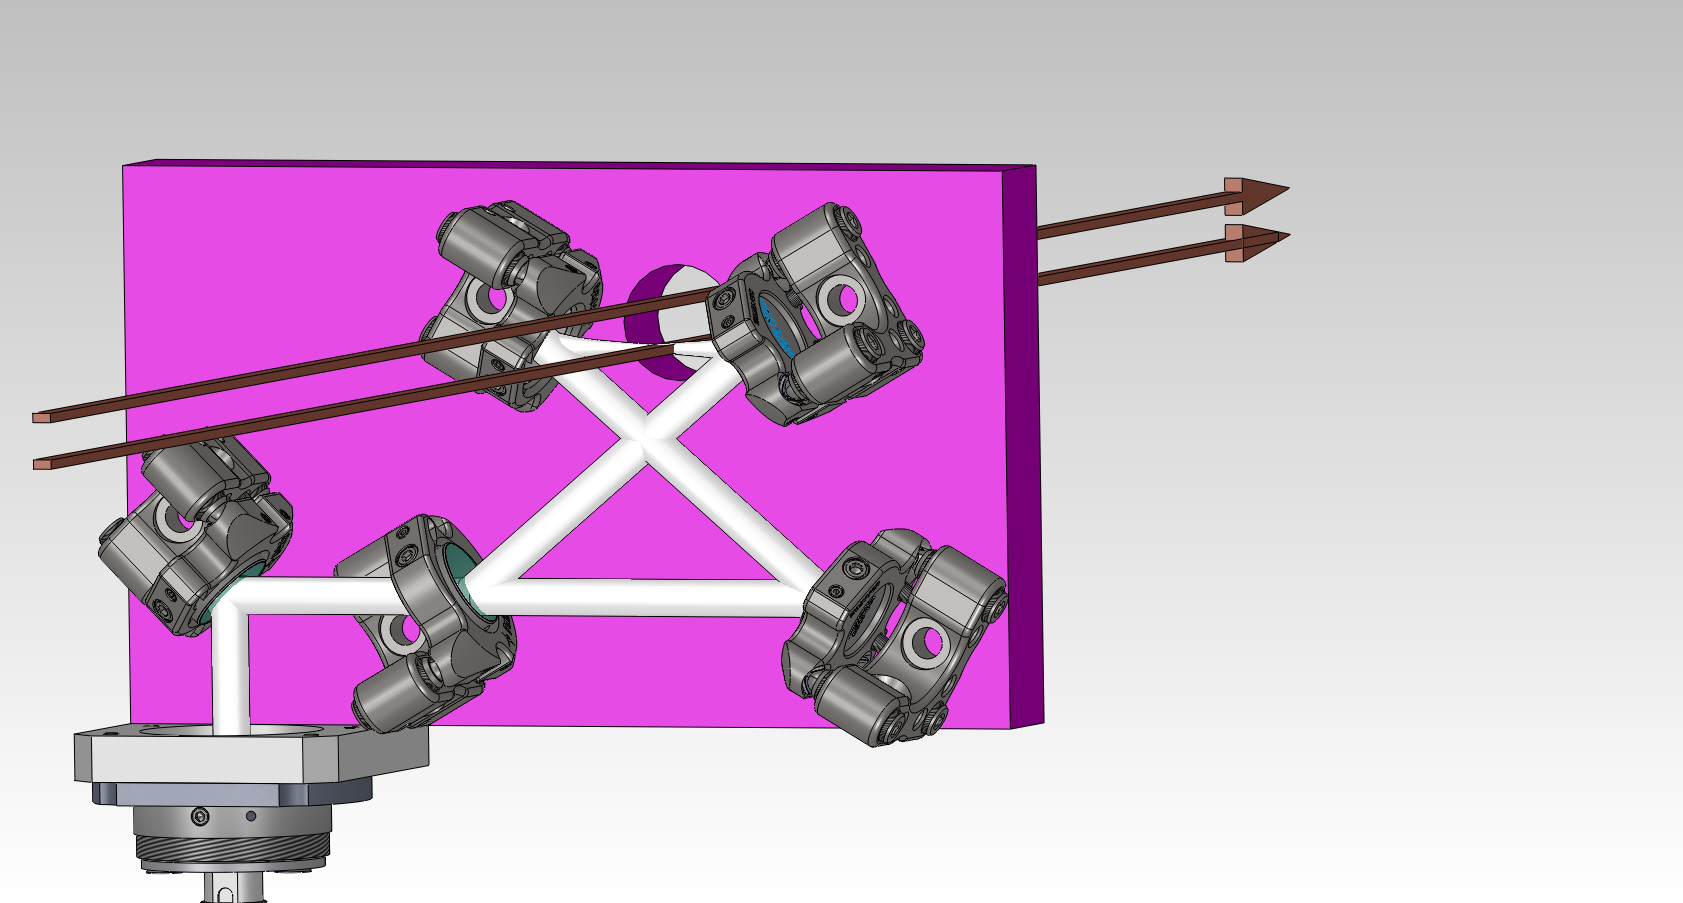
\includegraphics[width=.90\textwidth]{Figures/mzwCavityThruHole2.jpg}}
\caption[A power build-up cavity for improved measurements of $\lambdaZero$.]{\label{mzwCavityFig}A power build-up cavity for improved measurements of $\lambdaZero$. A power build-up cavity could provide 50-100 times larger phase shift for reasonable mirror reflectivities.}
\end{figure}

\begin{figure}
\centerline{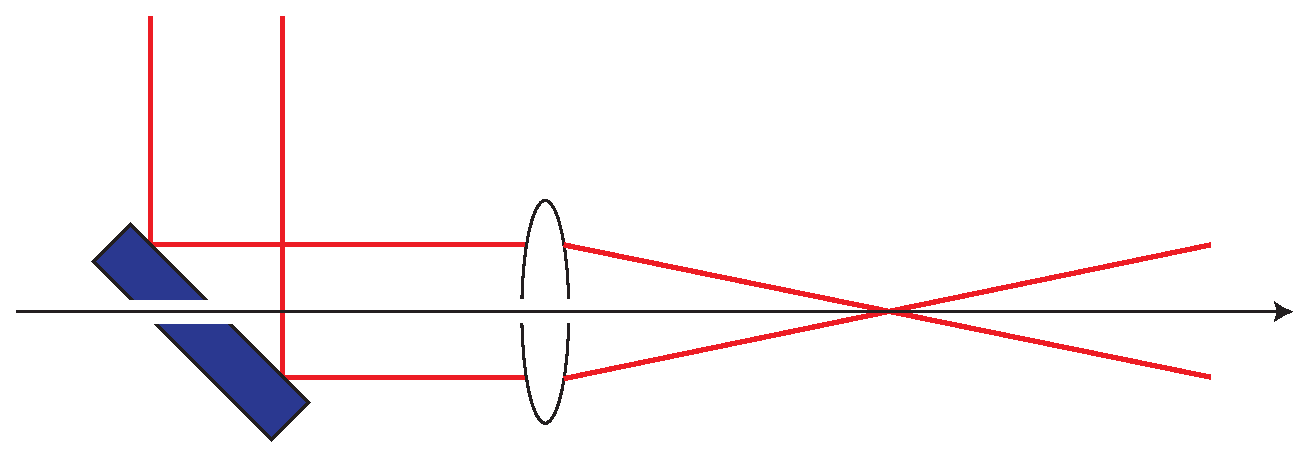
\includegraphics[width=.90\textwidth]{Figures/holeyMirror.eps}}
\caption[A coaxial atom-light interaction region for improved measurements of $\lambdaZero$.]{\label{mzwHoleyMirror}A coaxial atom-light interaction region for improved measurements of $\lambdaZero$. Light focused along the path of the atom beam could interact with the atoms for a significantly longer amount of time, leading to 50-100 times larger phase shifts. A small hole drilled in the mirror and lens would allow the atom beam to pass through while only reducing the total optical power by a few percent. The atoms would see significantly Doppler-shifted light, so an accurate measurement of the atom beam velocity is required in this system.}
\end{figure}


